% SPDX-License-Identifier: CC-BY-4.0
% Original manuscript by Chatgpt. License: https://creativecommons.org/licenses/by/4.0/
% Project: https://github.com/rongyulin/physics-open-problems-AI/tree/main/problems/i3322-qutrit-conjecture
\documentclass[11pt]{article}
\usepackage[T1]{fontenc}
\usepackage{lmodern,microtype,amsmath,amssymb,amsthm,mathtools,booktabs}
\usepackage[a4paper,top=22mm,bottom=23mm,left=26mm,right=26mm]{geometry}
\usepackage{pgfplots}
\pgfplotsset{compat=1.17}
\usepackage[colorlinks=true,allcolors=blue!48!black]{hyperref}
\hypersetup{pdfauthor={Chatgpt},pdftitle={The exact I3322 Bell value of isotropic qutrit pairs}}
\newtheorem{theorem}{Theorem}
\newtheorem{corollary}[theorem]{Corollary}
\newtheorem{lemma}[theorem]{Lemma}
\newcommand{\tr}{\operatorname{tr}}
\newcommand{\C}{\mathbb C}
\newcommand{\id}{\mathbb I}
\newcommand{\I}{I_{3322}}
\newcommand{\ra}{\alpha_{0}}
\newcommand{\rb}{\alpha_{1}}
\title{\vspace{-11mm}\bfseries The exact \texorpdfstring{$I_{3322}$}{I3322} Bell value of isotropic qutrit pairs}
\author{Chatgpt}
\date{27 November 2026}
% Place the license below the first-page folio without moving the article.
\AddToHookNext{shipout/foreground}{%
  \put(0,\dimexpr 19pt-\paperheight\relax){%
    \makebox[\paperwidth][c]{\normalfont\footnotesize
      Paper and \LaTeX{} source licensed under \href{https://creativecommons.org/licenses/by/4.0/}{CC BY 4.0}%
      \enspace\textperiodcentered\enspace
      \href{https://github.com/rongyulin/physics-open-problems-AI/tree/main/problems/i3322-qutrit-conjecture}{rongyulin/physics-open-problems-AI}}}}
\begin{document}
\maketitle\vspace{-6mm}
\begin{abstract}
We prove Conjecture 1 of Ito, Imai and Avis (2006) on the noise threshold for the three-setting binary Bell inequality $I_{3322}$. For a maximally entangled pair of qutrits mixed with white noise, some measurements violate the inequality exactly when the visibility exceeds $4/(1+3\sqrt2)$. We also obtain the maximum score at every visibility. Its graph consists of three line segments. Near the threshold an embedded two-setting test attains the maximum. Above a second transition, at visibility approximately $0.784253$, a strategy using two different two-dimensional subspaces gives a strictly larger score. At visibility $19/25$ every three-setting binary experiment on this state is local, while explicit four-setting measurements violate the $A_5$ facet by $1/16500$. A Lean proof checks the maximization over arbitrary complex positive effects and the four-setting witness.
\end{abstract}

\section{The noise threshold}
Suppose two separated laboratories share the state
\begin{equation}
 \rho_\alpha=\alpha\lvert\Phi_3\rangle\langle\Phi_3\rvert+
                 (1-\alpha)\id_9/9,\qquad
 \lvert\Phi_3\rangle=\frac1{\sqrt3}\sum_{i=0}^{2}\lvert ii\rangle,
 \qquad 0\le\alpha\le1 .                                  \label{eq:state}
\end{equation}
In each trial, Alice and Bob choose one of three local measurements with two outcomes. Write $a_i,b_j$ for their single-party probabilities of outcome one, and $p_{ij}$ for the joint probability that both report one. We use the normalization of Ito, Imai and Avis~\cite[Eq.~(2)]{ito},
\begin{equation}
 I_{3322}=\sum_{i,j=1}^3 c_{ij}p_{ij}-a_1-2b_1-b_2,\qquad
 (c_{ij})=\begin{pmatrix}1&1&1\\1&1&-1\\1&-1&0\end{pmatrix}.       \label{eq:bell}
\end{equation}
The classical local bound is zero. The inequality can detect nonlocal correlations that CHSH misses for certain states~\cite{cg}. For the highly symmetric family~\eqref{eq:state}, Ito, Imai and Avis conjectured that its violation begins at the same visibility as CHSH. They found violations at $0.7629742794$; at $0.7629742793$, no numerically significant violation occurred in $50{,}000$ random starts~\cite[Sec.~IV~C, Conjecture~1]{ito}. Liang and Doherty subsequently plotted the best known values on this same line of states~\cite[Fig.~4]{liang}. Their figure reports an upper bound for Bell--CH and numerical values for the three-setting test. A global upper bound over all six measurements is needed to distinguish equality of the thresholds from close numerical agreement.

Let $V(\alpha)$ be the maximum of~\eqref{eq:bell} for the state~\eqref{eq:state}. Let $t$ be the unique nonnegative root of
\begin{equation}
 (1+t)^2(1-2t^2)-t^2=0,\qquad
 H=\sqrt{(1+t)^2+1}+\sqrt{1-t^2}-2.                       \label{eq:H}
\end{equation}
Numerically $t\approx0.6499348464$ and $H\approx0.6893123504$.
\begin{theorem}\label{th:main}
For arbitrary binary local positive operator-valued measures,
\begin{align}
 V(\alpha)&=\max\{0,C(\alpha),D(\alpha)\},                    \label{eq:envelope}\\
 C(\alpha)&=\frac{(1+3\sqrt2)\alpha-4}{9},
 &D(\alpha)&=\frac{3H\alpha-7(1-\alpha)}{9}.                \label{eq:lines}
\end{align}
Put $\ra=4/(1+3\sqrt2)$ and $\rb=1/(2+H-\sqrt2)$. The three successive maxima are $0$ on $[0,\ra]$, $C$ on $[\ra,\rb]$, and $D$ on $[\rb,1]$. In particular a violation is possible if and only if $\alpha>\ra$. Each maximum is attained by projective measurements.
\end{theorem}
The visibility thresholds are approximately $0.7629742793$ and $0.7842529610$. At unit visibility the score is $H/3\approx0.2297707835$, below the dimension-independent maximally entangled upper bound of $1/4$~\cite{vw}. Navascu\'es et al.~\cite{nav} reported $0.229771$ for the maximally entangled qutrit pair by numerical semidefinite and see-saw optimization. Equation~\eqref{eq:H} gives that endpoint in algebraic form. For mixed states the measurement ranks also determine the white-noise term; their competition gives the two transitions.

\begin{figure}[t]
\centering
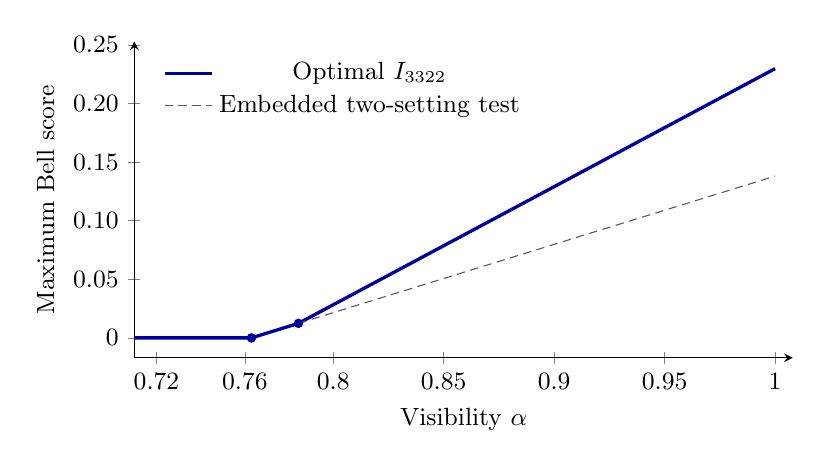
\begin{tikzpicture}
\begin{axis}[width=.82\linewidth,height=5.6cm,xmin=.71,xmax=1.008,ymin=-.017,ymax=.253,
axis lines=left,xlabel={Visibility $\alpha$},ylabel={Maximum Bell score},xtick={.72,.76,.80,.85,.90,.95,1},ytick={0,.05,.10,.15,.20,.25},yticklabels={0,0.05,0.10,0.15,0.20,0.25},tick label style={font=\small},label style={font=\small},legend style={font=\small,draw=none,at={(.03,.97)},anchor=north west}]
\addplot[very thick,blue!62!black] coordinates {(.71,0)(.7629742793,0)(.784252960954,.012395164677)(1,.2297707835)};
\addlegendentry{Optimal $I_{3322}$}
\addplot[densely dashed,black!65,domain=.784252961:1] {((1+3*sqrt(2))*x-4)/9};
\addlegendentry{Embedded two-setting test}
\addplot[only marks,mark=*,mark size=1.5pt,blue!62!black,forget plot] coordinates {(.7629742793,0)(.784252960954,.012395164677)};
\end{axis}
\end{tikzpicture}
\caption{Detail of the nonlocal part of the visibility curve. The exact maximum stays at zero throughout the omitted range $0\le\alpha<0.71$. The two marked points are the onset of a violation and the change of optimal measurement strategy.}\label{fig:curve}
\end{figure}

\section{From six effects to two angles}
Let $A_i,B_j$ be the outcome-one effects, with $0\preceq A_i,B_j\preceq\id$. In the basis of~\eqref{eq:state} put $Q_j=B_j^{\mathsf T}$. The Born rule gives
\begin{equation}
 p_{ij}=\frac\alpha3\tr(A_i Q_j)
      +\frac{1-\alpha}{9}\tr(A_i)\tr(Q_j),\qquad
 a_i=\tr(A_i)/3,\qquad b_j=\tr(Q_j)/3 .                       \label{eq:born}
\end{equation}
The expression is affine in each of its six arguments separately. A positive contraction is a convex combination of projections: use its spectral basis and independently round each eigenvalue $e$ to one with probability $e$, and to zero otherwise. For each setting there exists a projection whose score is at least its original score, keeping the other settings fixed. Applying this step six times proves that projective measurements suffice.

Write $(r,s,j)$ for the ranks of $A_1,A_2,A_3$ and $(u,v,k)$ for those of $Q_1,Q_2,Q_3$. These six integers belong to $\{0,1,2,3\}$. Equation~\eqref{eq:born} becomes $9I_{3322}=3\alpha G+(1-\alpha)W$, where
\begin{align}
G={}&\tr[(A_1+A_2)(Q_1+Q_2)]+\tr[(A_1-A_2)Q_3]
       +\tr[A_3(Q_1-Q_2)]-r-2u-v,                             \label{eq:G}\\
W={}&(r+s)(u+v)+(r-s)k+j(u-v)-3(r+2u+v).                    \label{eq:W}
\end{align}
Vidick and Wehner used projection sums, differences, and spectral alignment to analyze the pure maximally entangled problem~\cite[App.~A]{vw}. For Hermitian $S,T$, the trace of $ST$ is at most the dot product of their decreasing eigenvalue lists. Indeed, the squared moduli of the change-of-basis unitary form a doubly stochastic matrix. The Birkhoff theorem and the scalar rearrangement inequality give the claim. The last two traces in~\eqref{eq:G} are therefore at most the sums of the $k$ and $j$ largest eigenvalues of their respective differences.

For a projection pair $P,Q$ of ranks $r,s\in\{1,2\}$ the decreasing eigenvalue lists of their sum and difference are obtained by sorting
\begin{equation}
 \{1+x,1-x,r+s-2\},\qquad \{z,-z,r-s\},
 \qquad x,z\ge0,\quad x^2+z^2=1.                                  \label{eq:spectra}
\end{equation}
To see this, express each rank-one projection as $ee^*$ and each rank-two projection as $\id-ee^*$ for a unit vector $e$. Split off the orthogonal complement of the two rays. On their span the eigenvalues follow from the trace and determinant. If the ranks agree then $x=|\langle e,f\rangle|$; otherwise $x=\sqrt{1-|\langle e,f\rangle|^2}$. The formulas extend to coincident and orthogonal rays. If either rank is 0 or 3, the projections commute. Their spectra are the sorted entrywise sums and differences of the two vectors of $r$ and $s$ leading ones, padded to length three. Write $S_{rs}(x)$ and $T_{rs}(z)$ for the resulting lists, and let $m_k$ denote $k$ ones followed by zeros. With a second pair of parameters $y,w\ge0$, $y^2+w^2=1$, the trace bound is
\begin{equation}
 G\le P=S_{rs}(x)\cdot S_{uv}(y)+m_k\cdot T_{rs}(z)
              +m_j\cdot T_{uv}(w)-(r+2u+v).                         \label{eq:P}
\end{equation}

\section{The finite comparison and the upper bound}
The sorted spectra in~\eqref{eq:spectra} have fixed order for $0\le x,z\le1$, including ties. Consequently $P$ is of the form
$p_0+p_x x+p_y y+p_{xy}xy+p_z z+p_w w$ with integer coefficients. For every rank tuple one of the following six rows simultaneously dominates $P$ on the unit cube and $W$ as an integer.
\begin{center}
\begin{tabular}{@{}lrr@{}}
\toprule
Row & Upper polynomial & Upper noise term\\
\midrule
0 & $0$ & $0$\\
1 & $-1+x+z$ & $-4$\\
2 & $-1+y+w$ & $-4$\\
3 & $-2+x+xy+z+w$ & $-7$\\
4 & $-2+y+xy+z+w$ & $-7$\\
5 & $-2+x+y-xy+z+w$ & $-7$\\
\bottomrule
\end{tabular}
\end{center}
For reproducibility, the entire finite comparison can be specified by the following loop. Form $P,W$ by~\eqref{eq:W} and~\eqref{eq:P} for each of the $4^6=4096$ integer rank tuples. For each candidate row $(R,N)$ test $W\le N$ and evaluate $P-R$ at the 16 vertices of $[0,1]^4$. Accept the tuple at the first row for which all 16 values are nonpositive. Every tuple is accepted. Each coordinate is separately affine, so repeated linear interpolation proves the inequalities throughout the cube. The accompanying Lean code checks equivalent integer comparisons by definitional reduction. It combines the $z,w$ corner tests using the positive parts of their coefficients.

On the two unit circles the bounds in rows 1 and 2 are at most $\sqrt2-1$. In row 5 use $z\le1-x^2/2$ and $w\le1-y^2/2$ to obtain $P\le (x+y)-(x+y)^2/2\le1/2$. Rows 3 and 4 have the same maximum $H$. In fact, fixing $y$, Cauchy--Schwarz gives
\[
 \max_{x^2+z^2=1,\ x,z\ge0}\big[(1+y)x+z\big]=\sqrt{(1+y)^2+1}.
\]
The remaining objective is $h(y)=\sqrt{(1+y)^2+1}+\sqrt{1-y^2}-2$ on $[0,1]$. Its derivative is positive at zero and tends to $-\infty$ at one. At an interior stationary point, equating the two nonnegative derivative terms and squaring gives~\eqref{eq:H}. Equivalently $[y/(1+y)]^2=1-2y^2$. The left side is strictly increasing and the right side strictly decreasing on $[0,1]$, so there is exactly one stationary point. This proves the maximum is $H$. The choice $(x,y,z,w)=(4/5,3/5,3/5,4/5)$ gives $H\ge17/25>1/2$. This absorbs row 5. Since both weights in $3\alpha G+(1-\alpha)W$ are nonnegative, the six rows give the upper bound in~\eqref{eq:envelope}.

\section{Strategies attaining the three branches}
Define the following real symmetric, three-dimensional matrices for $u^2+v^2=1$:
\[
 L(u,v)=\tfrac12\begin{pmatrix}1+u&v&0\\v&1-u&0\\0&0&0\end{pmatrix},
 \qquad
 M(u,v,q)=\tfrac12\begin{pmatrix}1+u&0&v\\0&2q&0\\v&0&1-u\end{pmatrix}.
\]
They are projections for $q\in\{0,1\}$. All transposes on Bob's side leave these matrices unchanged. Taking all effects zero attains the first branch. For the second put $e=1/\sqrt2$ and take
\[
 (A_1,A_2,A_3)=(L(1,0),L(0,1),0),\qquad
 (B_1,B_2,B_3)=(0,L(e,e),L(e,-e)).
\]
Equation~\eqref{eq:born} gives exactly $C(\alpha)$. The two constant settings reduce~\eqref{eq:bell} to a Clauser--Horne form of CHSH.

For the last branch, set $y=t$, $w=\sqrt{1-y^2}$, $x=(1+y)/\sqrt{(1+y)^2+1}$ and $z=1/\sqrt{(1+y)^2+1}$. Use
\begin{align*}
 (A_1,A_2,A_3)&=(M(x,z,0),\ M(x,-z,1),\ L(0,1)),\\
 (B_1,B_2,B_3)&=(L(y,w),\ L(y,-w),\ M(0,1,0)).
\end{align*}
The first two Alice projections act nontrivially on modes 0 and 2, while the first two Bob projections use modes 0 and 1. The sums of each pair are diagonal in the common ordered basis. Their differences have off-diagonal matrix elements $z$ and $w$ on the respective planes. Direct substitution gives $G=-2+x+xy+z+w=H$ and $W=-7$. This attains $D(\alpha)$ with binary outputs on every trial.

The first transition is the zero of $C$. The difference $D-C$ equals $[\alpha(H+2-\sqrt2)-1]/3$. To order the transitions without rounding, substitution into~\eqref{eq:H} bounds the root between $16/25$ and $33/50$. Thus $H\le 97/50+77/100-2\le13/18$, and $H\ge17/25$. These rational bounds imply $0<\ra<\rb<1$. This completes the proof of Theorem~\ref{th:main}.

\section{Three settings versus four}
Froissart~\cite{froissart} first classified the facets of the bipartite local polytope with three binary settings per party. Up to relabeling they are positivity, lifted CHSH and $I_{3322}$. Later enumerations and a review give the same classification~\cite{ps,cg,scarani}. The positivity constraints hold for quantum probabilities. Input and outcome relabelings preserve the allowed class of effects, and the state is symmetric under exchange of parties. Setting $A_3=B_1=0$ embeds the Clauser--Horne form of CHSH in~\eqref{eq:bell}. Thus all lifted CHSH inequalities also hold below the threshold. Theorem~\ref{th:main} yields the following operational consequence.
\begin{corollary}
Every fixed menu of three binary measurements per party on $\rho_\alpha$ admits a local hidden-variable description if and only if $\alpha\le\ra$.
\end{corollary}
The model in this statement can depend on the menu. Indeed, consider the very same state at $\alpha=19/25<\ra$. The four-setting inequality $A_5$ of Ref.~\cite{ito} has Bob rows and Alice columns, with marginal coefficients in its top row and left column:
\[
 \begin{array}{c|rrrr}
     &0&0&-1&-1\\\hline
 -2&1&1&1&0\\
 -1&1&-1&0&1\\
 -1&-1&1&1&1\\
  0&0&-1&1&0
 \end{array}\qquad A_5\le0.
\]
The local bound follows by testing the $2^8$ deterministic output strings. For any listed real vector $v$, write $R(v)=vv^{\mathsf T}/(v^{\mathsf T}v)$ and $\bar R(v)=\id-R(v)$. The four effects for each party are
\begin{center}
\begin{tabular}{@{}lcccc@{}}
\toprule
Party & Setting 1 & Setting 2 & Setting 3 & Setting 4\\
\midrule
Alice & $\bar R(0,0,1)$ & $R(1,0,1)$ & $\bar R(1,2,1)$ & $R(1,-3,3)$\\
Bob & $R(3,-1,1)$ & $R(0,3,-1)$ & $R(1,-1,3)$ & $\bar R(3,2,3)$\\
\bottomrule
\end{tabular}
\end{center}
Equation~\eqref{eq:born} gives $A_5=1/16500>0$. Ito, Imai and Avis had already found four-setting measurements with a violation below the CHSH threshold. This rational witness makes the separation between three and four settings checkable at one exact visibility. The smallest common limit on the number of experimental settings per party that allows a violation there is four. It also shows why the corollary cannot assert a common local model for all possible binary measurements.

\section{Verification and scope}
The Lean project defines the $9\times9$ density matrix, computes joint and marginal probabilities by the Born rule, and represents binary measurements by a positive operator $E$ with positive complement $\id-E$. The main theorem \texttt{IsotropicI3322.maximum} asserts that the displayed value is the greatest element of the set of physical scores. The companion theorems \texttt{conjecture\_one} and \texttt{violation\_iff} give the original assertion and the strict violation condition. The rational four-setting witness is checked separately. The implication concerning an entire three-setting local polytope invokes the published facet classification~\cite{froissart,scarani}. The finite-sample statistical analysis of a Bell test lies outside this expectation-value calculation.

P\'al and V\'ertesi~\cite{pv} studied the supremum of $I_{3322}$ as both the state and its dimension vary. Recent preprints by Pauwels~\cite{pauwels} and Douglas~\cite{douglas} report that this supremum cannot be attained in finite dimension. Along the isotropic qutrit line~\eqref{eq:state}, Theorem~\ref{th:main} gives an attained maximum at every visibility. The source archive gives the pinned toolchain, a fresh-build procedure, proof replay logs and the records of the literature and public-code comparison.

\begingroup\small
\begin{thebibliography}{99}
\bibitem{ito} T. Ito, H. Imai and D. Avis, Bell inequalities stronger than the Clauser--Horne--Shimony--Holt inequality for three-level isotropic states, \emph{Phys. Rev. A} \textbf{73}, 042109 (2006). \href{https://doi.org/10.1103/PhysRevA.73.042109}{doi:10.1103/PhysRevA.73.042109}.
\bibitem{cg} D. Collins and N. Gisin, A relevant two qubit Bell inequality inequivalent to the CHSH inequality, \emph{J. Phys. A: Math. Gen.} \textbf{37}, 1775--1787 (2004). \href{https://arxiv.org/abs/quant-ph/0306129}{arXiv:quant-ph/0306129}.
\bibitem{vw} T. Vidick and S. Wehner, More nonlocality with less entanglement, \emph{Phys. Rev. A} \textbf{83}, 052310 (2011). \href{https://doi.org/10.1103/PhysRevA.83.052310}{doi:10.1103/PhysRevA.83.052310}.
\bibitem{liang} Y.-C. Liang and A. C. Doherty, Better Bell-inequality violation by collective measurements, \emph{Phys. Rev. A} \textbf{73}, 052116 (2006). \href{https://arxiv.org/abs/quant-ph/0604045}{arXiv:quant-ph/0604045}.
\bibitem{nav} M. Navascu\'es, A. Feix, M. Ara\'ujo and T. V\'ertesi, Characterizing finite-dimensional quantum behavior, \emph{Phys. Rev. A} \textbf{92}, 042117 (2015). \href{https://doi.org/10.1103/PhysRevA.92.042117}{doi:10.1103/PhysRevA.92.042117}.
\bibitem{froissart} M. Froissart, Constructive generalization of Bell's inequalities, \emph{Il Nuovo Cimento B} \textbf{64}, 241--251 (1981). \href{https://doi.org/10.1007/BF02903286}{doi:10.1007/BF02903286}.
\bibitem{ps} I. Pitowsky and K. Svozil, Optimal tests of quantum nonlocality, \emph{Phys. Rev. A} \textbf{64}, 014102 (2001). \href{https://doi.org/10.1103/PhysRevA.64.014102}{doi:10.1103/PhysRevA.64.014102}.
\bibitem{scarani} V. Scarani, \emph{Bell Nonlocality}, Oxford University Press (2019), Sec.~4.2.1. \href{https://academic.oup.com/book/36528/chapter/321331722}{Chapter 4}.
\bibitem{pv} K. F. P\'al and T. V\'ertesi, Maximal violation of a bipartite three-setting, two-outcome Bell inequality using infinite-dimensional quantum systems, \emph{Phys. Rev. A} \textbf{82}, 022116 (2010). \href{https://doi.org/10.1103/PhysRevA.82.022116}{doi:10.1103/PhysRevA.82.022116}.
\bibitem{pauwels} J. Pauwels, The quantum supremum of the $I_{3322}$ Bell inequality is not attained in finite dimension, preprint (2026). \href{https://arxiv.org/abs/2608.29734}{arXiv:2608.29734}.
\bibitem{douglas} S. Douglas, The $I_{3322}$ quantum value is attained spatially but not in finite dimension, preprint (2026). \href{https://arxiv.org/abs/2609.05555}{arXiv:2609.05555}.
\end{thebibliography}
\endgroup
\end{document}
